% Diese Zeile bitte -nicht- aendern.\pgfplotsset{compat=1.15}
\documentclass[course=erap]{aspdoc}
\graphicspath{ {./} }

%%%%%%%%%%%%%%%%%%%%%%%%%%%%%%%%%
%% TODO: Ersetzen Sie in den folgenden Zeilen die entsprechenden -Texte-
%% mit den richtigen Werten.
\newcommand{\theGroup}{140} % Beispiel: 42
\newcommand{\theNumber}{A208} % Beispiel: A123
\author{Tianhao Gu \and Zhongfang Wang \and Julien Escaig}
\date{Wintersemester 2023/24} % Beispiel: Wintersemester 2019/20
%%%%%%%%%%%%%%%%%%%%%%%%%%%%%%%%%

% Diese Zeile bitte -nicht- aendern.
\title{Gruppe \theGroup{} -- Abgabe zu Aufgabe \theNumber}

% document content
\begin{document}
\maketitle

% einleitung content
\section{Einleitung}
\par
Im Rahmen dieser Projektaufgabe befassen wir uns mit der Herausforderung, einen Algorithmus in der Programmiersprache C zu entwerfen, der ein farbliches Bild in ein Graustufenbild transformiert und im Anschluss die Helligkeit des Graustufenbilds anpasst. Der Algorithmus lässt sich also in zwei distinkte Phasen unterteilen.

\par
Die erste Phase ist die Graustufenkodierung. In diesem Teil wird als Input eine PPM Datei erwartet. Diese besteht aus einem Header mit Metadaten, worauf die Pixel-Informationen folgen. Im Datenteil der PPM Datei gibt es für jeden Pixel genau drei Werte, die jeweils die Stärke der Farben Rot, Grün und Blau speichern. Je größer der Wert desto stärker ist die Farbe in einem bestimmten Pixel vertreten (Siehe siehe Abb.1)

% \par
% \includegraphics[width=\textwidth]{Bilder/ppm1.png}

\par
Im ersten Teil des Algorithmus wird nun diese PPM Datei in eine Bilddatei im PGM Format verwandelt. Eine PGM Datei besitzt ebenfalls einen Header mit Metadaten und darauf folgende Informationen über die Pixel. Da eine PGM Datei nur Graustufen darstellt, wird pro Pixel jeweils nur ein Integer-Wert gespeichert.(siehe Abb2)

% \par
% includegraphics[width=\textwidth]{Bilder/pgm1.png}

\par
Für die Verwandlung von einem Farbbild (PPM) in ein Graustufenbild (PGM) werden jeweils die 3 Werte pro Farbpixel zu einem Graupixel-Wert zusammengefasst. Diese Transformation ist im Grunde ein gewichteter Durchschnitt, der durch die folgende Formel berechnet wird:

\begin{center}
${D(x,y)=\frac{a*R+b*G+c*B}{a+b+c}}$
\end{center}

\par
Kommen wir nun zur zweiten Phase des Algorithmus: Die Anpassung der Helligkeit. Dies passiert durch die sogenannte Gammakorrektur. Um diese besser verstehen zu können, betrachten wir erstmal eine simple Grafik (Abb3):

% \par
% \includegraphics[width=\textwidth]{Bilder/gammakorrektur.png}

\par
Das mittlere Bild ist das originale Bild. Wie man leicht erkennen kann, ist nach der Gammakorrektur das rechte Bild dunkler und das linke Bild heller. Die Auswirkung der Gammakorrektur hängt also von der Wahl des y Parameters (auch Gammawert genannt) ab.

\par
Bei diesem Algorithmus wird die Gammakorrektur durch folgende mathematische Formel bestimmt:

\begin{center}
${D'(x,y)={\left( \frac{D(x,y)}{255} \right)}^{\gamma}*255}$
\end{center}

\par
Die Werte D'(x,y) ergeben die Intensität der Graustufenkodierung für alle Pixel (x,y). Bei einem Gammawert kleiner 1, ist D'(x,y) stets kleiner als D(x,y) und das Bild wird heller. Bei einem Gammawert größer 1, ist D'(x,y) stets größer ist als D(x,y) und das Bild wird dunkler.

\par
Eine weitere Herausforderung dieses Projekt war es diese Gammakorrektur-Formel ohne das Verwenden der Power-Funktion aus der Math Lib zu implementieren. Dafür wurde eine Algorithmus entworfen der nur mit grundlegenden, arithmetischen Operqationen und der Hilfe der Taylorreihe den Wert der Gammakorrektur approximentiert. 



% solution content
\section{Lösungsansatz}
\par
Unser Programm betrachtet aus der Perspektive einer Black Box, nimmt ein Bild im 24bpp PPM-Format entgegen und gibt dieses Bild nach einer Graustufen Konvertierung und Gamma-Korrektur aus, wobei es im PGM-Format gespeichert wird. PGM (Portable Graymap Format) und PPM (Portable Pixmap Format) sind Teil des Netpbm-Bildformats. PPM ist ein einfaches Dateiformat für Farbbitmapbilder. 24bpp (Bits pro Pixel) bedeutet, dass jedes Pixel mit 24 Bits repräsentiert wird, 8 Bits für jede Farbe (nämlich Rot R, Grün G, Blau B). 

\par
Unser Programm akzeptiert nur P6-Typ PPM-Eingaben. P6 bezieht sich auf das Binärformat, das im Gegensatz zum ASCII-basierten P3-Typ kompakter und schneller in der Lese-/Schreibgeschwindigkeit ist.Unten ist ein einfaches Beispiel, das dem folgenden Bild entspricht(P6 PPM).

% graph 
\begin{figure}[h]
\begin{minipage}{0.45\textwidth}
\centering
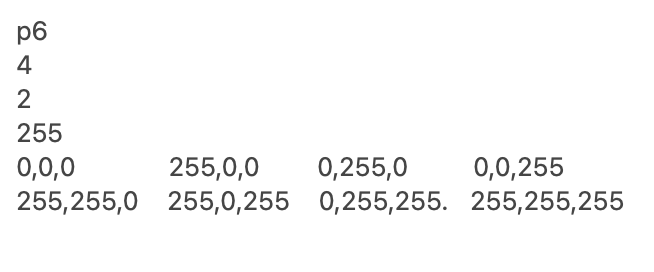
\includegraphics[width=\textwidth]{Bilder/demograph.png}
\caption{ein Beispiel für P6 PPM}
\end{minipage}
\hfill
\begin{minipage}{0.45\textwidth}
\centering
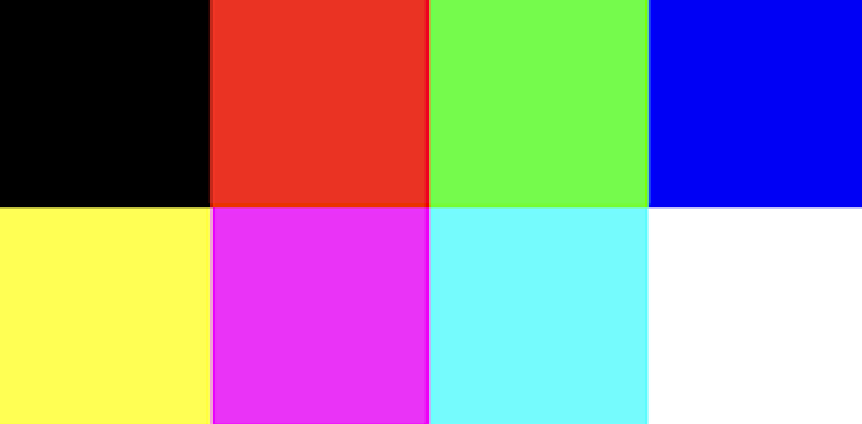
\includegraphics[width=\textwidth]{Bilder/demograph.ppm.png}
\caption{erzeugt durch den Beispielcode}
\end{minipage}
\end{figure}


\par
Wir verwenden eine Formel für die Graustufen Konvertierung, um einen gewichteten Durchschnittswert der R-, G- und B-Werte jedes Pixels zu ermitteln und diesen in der PGM zu speichern.Wir wählen PGM, weil es Graustufenbilder speichert. Jeder Pixelwert liegt zwischen 0 und dem maximalen Grauwert, wobei 0 normalerweise Schwarz darstellt, der maximale Grauwert Weiß und die Zwischenwerte verschiedene Grautöne. Der maximale Grauwert ist üblicherweise 255 (8 Bits).Hier muss aber beachtet werden, wie die "Gewichte" von RGB gewählt werden. 

\par
Aufgrund der Eigenschaften des menschlichen visuellen Systems (HVS), wie Empfindlichkeit gegenüber verschiedenen Farben und Helligkeiten, könnten diese die optimalen Werte der Parameter beeinflussen. Beispielsweise ist das menschliche Auge empfindlicher für Grün als für Rot und Blau, so dass bei der Umwandlung von Farbbildern in Graustufenbilder das Gewicht der grünen Komponente größer sein könnte als das der roten und blauen Komponenten.Wir setzen die Standardwerte von a, b, c wie folgt fest:a=0.2126 b=0.7152 c=0.0722 . Dann mitteln wir die RGB-Werte gewichtet.Das Graustufenbild von Bild (a), das durch Anwendung der Standardwerte a,b,c erhalten wird, sieht wie folgt aus:

% graph
\begin{figure}[h]
    \centering
    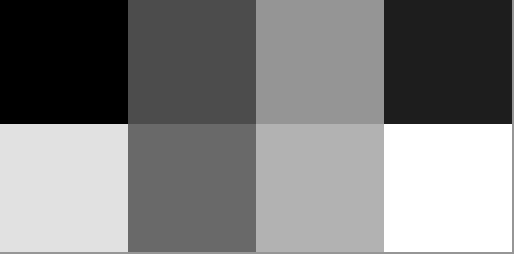
\includegraphics[width=0.5\textwidth]{Bilder/gamma1.pgm.png}
    \caption{Graustufen Konvertierung von Abbildung2}
    \end{figure}

\par
Wir haben die Aufgabe grundsätzlich abgeschlossen, aber um die menschliche Sicht anzupassen, führen wir eine Gammakorrektur durch. Gammakorrektur ist eine Technik zur Anpassung der Helligkeit oder des Kontrastes von Bildern oder Videos. Ihr Zweck besteht darin, dass das Bild im menschlichen Sehsystem natürlicher wirkt. Der Gammawert ist der Parameter, der diese Korrektur steuert. Es ist eine positive Zahl, die normalerweise zwischen 1,0 und 2,2 liegt.
\par
Unser Programm ist jedoch in der Lage, alle Gammawerte größer als 0 zu empfangen.Also je höher der Gammawert, desto höher der Kontrast des Bildes und desto größer die Unterschiede zwischen hellen und dunklen Bereichen. Umgekehrt ist der Kontrast des Bildes bei einem niedrigeren Gammawert geringer und die Unterschiede zwischen hellen und dunklen Bereichen sind geringer. Wir wenden die folgende Formel für jeden Graustufenwert an, wobei Gamma auf 1 gesetzt wird, wenn der Benutzer es nicht angibt:
% gamma fomular

\par
Unten stehen drei Vergleiche für die Graustufenbild Abbildung3: Gammawert auf 0.1 eingestellt, ohne Gammakorrektur, Gamma-Wert auf 10 eingestellt.
% three graph
% graph
\begin{figure}[h]
\begin{minipage}{0.3\textwidth}
\centering
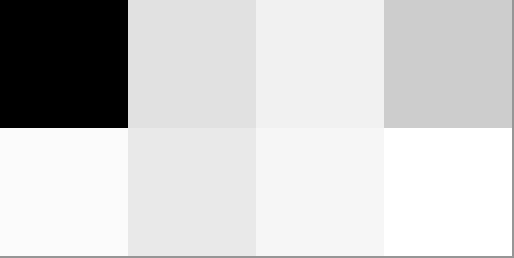
\includegraphics[width=\textwidth]{Bilder/gamma0.1.pgm.png}
\caption{Gamma=0.1}
\end{minipage}
\hfill
\begin{minipage}{0.3\textwidth}
\centering
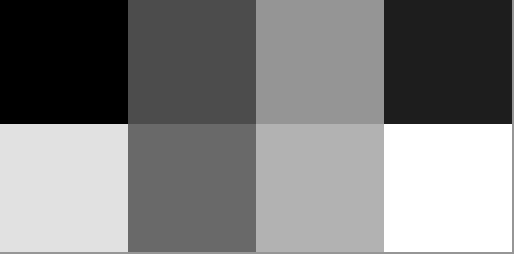
\includegraphics[width=\textwidth]{Bilder/gamma1.pgm.png}
\caption{Gamma=1}
\end{minipage}
\hfill
\begin{minipage}{0.3\textwidth}
\centering

\includegraphics[width=\textwidth]{Bilder/gamma10.pgm.png}
\caption{Gamma=10}
\end{minipage}
\end{figure}


% TODO: Je nach Aufgabenstellung einen der Begriffe wählen
\section{Genauigkeit}
\par
In diesem Teil wird die Genauigkeit bzw. Korrektheit des Algorithmus untersucht. Dafür ist erst einmal zu klären, welches der beiden Konzepte bei dieser Problemstellung sinnvoll anwendbar ist.

\par
Da der Algorithmus zwischendurch mit Float-Werten arbeitet, kann es zu Ungenauigkeiten kommen, da nicht alle Zahlen als Float darstellbar sind. Der maximale Fehler bei 32 bit Float beträgt ungefähr xxx. Diese mögliche Ungenauigkeit wird bei der Gammakorrektur noch verstärkt (Die Ungenauigkeit hängt zudem noch von der internen Implementation der arithmetischen Operationen ab). Obwohl der Fehler immer noch sehr klein ist, kann es bei der Rundung zu Integern zu unterschiedlichen Werten kommen. Für das menschliche Auge macht es keinen Unterschied. Die Bilder sehen identisch aus, obwohl nicht alle Integerwerte in der PGM Datei übereinstimmen. Aus diesen Gründen macht es Sinn, das resultierende Bild auf Genauigkeit anstatt auf Korrektheit zu überprüfen.

\par
Im Folgenden werden die 2 Teile des Programms erstmal getrennt voneinander auf Genauigkeit geprüft. Beginnen wir also mit der Graustufenkodierung.

\par
Um unsere Implementierung der Graustufenkodierung auf Genauigkeit zu überprüfen, verwenden wir die von Netpbm bereitgestellte Funktion “ppmtopgm” als Referenz. Dazu haben wir eine Funktion entworfen die zwei PGM Dateien als Input nimmt und die betragsmäßige Abweichung über alle Pixel berechnet. Die Grafik1 zeigt unsere Ergebnisse für verschiedene PGM Dateien unterschiedlicher Größe.

\par
Diese Abweichungen können jedoch niemals mit bloßem Auge erkannt werden, wie Abbildung 4 demonstriert.

\par
Nun folgt die Genauigkeitsanalyse des zweiten Teils des Programms. Diese wird erneut in mehrere Teile aufgeteilt. Dafür überprüfen wir die Genauigkeit der Pow()-Funktion, die der Taylorreihe und abschließend noch die der SIMD Implementation. Als Referenz der für das Resultat nach der Gammakorrektur verwenden wir die Funktion “gammakorrekt” des Netpbm Packages. In der Grafik2 kann man nun die Abweichung unserer Implementierung von der Netpbm-Implentierung beobachten.

\par
Nun beschäftigen wir uns mit der Genauigkeit der Taylorreihe. Die Taylorreihe ist eine Approximation, die erst bei unendlich vielen Gliedern exakt wird. In unserer Implementation der Taylorreihe brechen wir die Berechnung der Taylorreihe ab, sobald das nächste Reihenglied betragsmäßig kleiner als 0.00000001 ist. Dies lässt vermuten, dass die Abweichung bei dieser Implementation größer sein wird, als beim Verwenden der Pow-Funktion. In Grafik3 ist klar zu erkennen, dass es durch die Approximation der Taylorreihe insgesamt zu einer höheren Abweichung kommt.


\par
Abschließend betrachten wir noch die SIMD Implementation. Es ist zu erwarten, dass es zu keinem Unterschied in der Abweichung kommt, da die gleichen Operationen auf den gleichen Variablen durchgeführt werden. Grafik4 unterstreicht diese Hypothese.

\section{Performanzanalyse}


\section{Zusammenfassung und Ausblick}
\par
Bei\cite{vmintromiami} diesem Projekt ging es darum, eine Graustufen-Kodierung und Gammakorrektur selber zu programmieren. Das Umsetzen der Graustufen-Kodierung war relativ einfach, genau wie die Implementierung mit der Pow-Funktion. Die Aufgabe erhielt eine neue Stufe an Komplexität, sobald es zur Implementierung mit der Taylorreihe und der SIMD Implementierung kommt. Die Taylorreihe führt zu einer geringeren Genauigkeit. Die SIMD-Funktion hat zu einer höhere Performanz von etwa … Prozent geführt. Abschließend kann man sagen, dass dieses Projekt einen interessanten Einblick in verschiedene Bildformate, das Approximieren mit Hilfe der Taylorreihe und das Optimieren mit Hilfe von SIMD-Intrinsics geliefert hat.

% TODO: Fuegen Sie Ihre Quellen der Datei Ausarbeitung.bib hinzu
% Referenzieren Sie diese dann mit \cite{}.
% Beispiel: CR2 ist ein Register der x86-Architektur~\cite{intel2017man}.
\bibliographystyle{plain}
\bibliography{Ausarbeitung}

\end{document}



